
\section{Literature Review}
\subsection{Sentiment Analysis Tools}

\todo{PYTHON}

Many existing sentiment analysis tools are tailored towards market research for businesses, so focus on providing opinion mining tools for social media. This means that they focus on extracting the valence, and the subject that is being talked about in the text. In terms of obtaining an emotion from a piece of text, this is just limited to retrieving how positive or negative it is. Emotion can be argued as more than just a binary sentiment, so there is an interest into whether more information about the text's mood can be analysed. 

There seems to be very little existing work which tries to use semantic analysis to predict more than just the valence of text, as most existing work is only considering how positive or negative the input is. Attempting to predict a more descriptive form of the emotion of the input will be a challenge.

When analysing the positivity and negativity of tweets, using a lexicon based approach as well as machine learning approaches have been used \cite{kolchyna2015twitter} to great effect. In this case, a combination of the two has proved to be the most effective. Investigating whether these approaches work just as well when taking into account more than just the valence of the text will be the majority of the work on this project.

Existing sentiment analysis research processes the data a large amount before any machine learning is done on it, for example by removing all the words which lie exactly in the middle of the valence scale.  \cite{kolchyna2015twitter} The different pre-processing methods will also be compared during this project.


\subsection{Sentiment Representation structures}

\subsubsection{Ekman's Six Basic Emotions}

There is no universally accepted model for representing emotion, but a standard for classifying emotions in a categorical model is using Ekmans six basic emotions \cite{Ekman}. These are identified as Anger, Disgust, Fear, Happiness, Sadness and Surprise. Being able to use these fundamental emotions to represent the sentiment of a text allows for more insight into the emotions around it. Since there are only six discrete classes in which emotions can be placed, this can be argued to be very subjective when classifying however \cite{emoBank}.

\subsubsection{Valence}
A very common way to classify phrases and sentences in sentiment analysis is to analyse the valence of the text \cite{frijda1986emotions}.

The valence of a piece of text is how positive or negative the emotion behind it is. An example of a sentence with a high valence would be "I am feeling very happy, I'm having a great day!", compared to a low valence, "I am having a terrible day, everything is going wrong". 

As this is a dimensional model, where values chosen could be hypothetically infinite this can represent a wider range than just six classes such as Ekmans emotions, however only measuring the positivity or negativity of a text does not provide much insight into it.
Using valence in a machine learning context is very useful though, as commonly the valence values can be put into discrete binary classes, positive or negative, and is a good base to start from.

\subsubsection{Valence Arousal Dominance Structure}

The Valence-Arousal-Dominance (VAD) structure introduced in 1974 \cite{VAD} provides a 3D representation for emotions, with each variable being defined as follows:
\begin{itemize}
    \item Valence- How positive or negative the statement is.
    \item Arousal- Degree of calmness or excitement, the energy of the statement. 
    \item Dominance- Degree of control over a situation.
\end{itemize}

Using VAD values allow for easy representation into the Ekman six basic emotions, as although there is no standard on the exact VAD values to use for each emotion, the primary dataset that will be used references values given by Russell and Mehrabian \cite{VADMapping}.

Using the VAD structure to represent sentiment in this project was ideal, as it allows for much more description of emotion in text \cite{emotionPerspective}, and having numeric values means its easy to work with.


\subsection{Available Data}
There are two suitable datasets for this task, which will both be used to train the sentiment analysis tool on.

\subsubsection{Affective Ratings for Words}
To increase the range of data to train with, a dataset that contains VAD values for almost 14,000 English words\cite{wordsData} is also being incorporated, and can help balance out unnecessarily strongly weighted words by reclassifying them into a more appropriate emotional state. The issue with having only the individual words rated with VAD values means that the context in which the words are used can be lost, so this is a case where using a bag-of-words method for splitting up the sentences may not be the most appropriate.

\subsubsection{EmoBank}
This dataset is the most important one for this project, as it contains 10,000 English sentences covering multiple genres, all annotated with their own VAD values \cite{emoBank}.

This dataset contains VAD values for each piece of text from both writer and the reader of the text, but due to the findings in \cite{emoBank} only the values given by the reader will be used, as it is concluded that this perspective has higher emotionality and therefore they should be easier to train with.

\todo{mention the size of the dataset not being that large}





\subsection{Data Pre-Processing Approaches}

During investigation of existing sentiment analysis tools, Ricky Kim's series on investigating sentiment in twitter data \cite{towardsDS} explores areas in which data can be pre processed so that predictions can be optimised, and the two main ways that this experiment is done is by varying the N-Gram value and number of features supplied to the model.

\todo{ngram diagram}

During these experiments, unigrams, bigrams and trigrams are compared and analysed over a feature range of 10000 to 100001. These experiments are done over a totally balanced dataset, with 50\% of the data being classed as having a positive valence, and the other 50\% with a negative one, and produce results as shown in figure that imply that these methods are worth investigating.


\begin{figure}[h]
\caption{Results from Ricky Kim's investigation for N-Gram and Number of Features selection for valence analysis over the Sentiment 140 Dataset \cite{go2016sentiment140}}
\centering
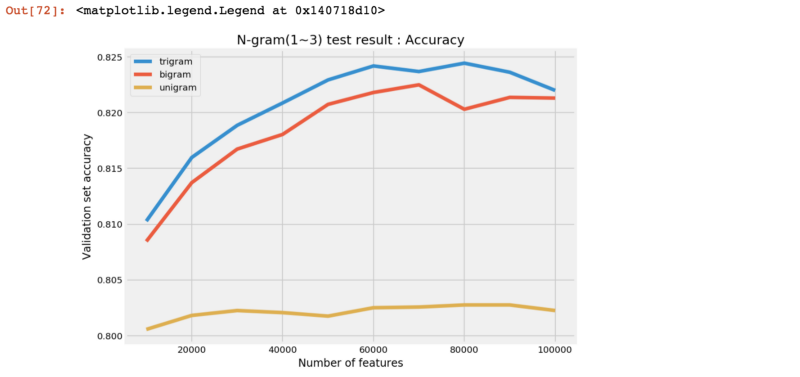
\includegraphics[scale=0.5]{litImgs/towardsDSNgramNFeatures.png}
\end{figure}


\subsection{Model building approaches}

There has been a little research into using a multi-dimensional VAD structure to investigate sentiment, primarily investigating whether using a VAD structure could be used to help identify burnout in software developers by analysing the messages in development repositories. \cite{mantyla2016mining} In this case, a correlation was found between each of the dimensions and different issues raised within the input text, meaning that there is an argument for using multiple dimensions to help understand textual data to a greater degree. An issue with this research is that they only used a word based lexicon where each word individual word was assigned a value. This loses the context in which each word is being used in, and by using a VAD dataset for sentences to train over this issue will be mitigated.


Generally for semantic analysis machine learning models, Logistic Regression is a popular classifier due to it being linear and scalable for large datasets \cite{towardsDS}, so this is the model that will be initially used for creating the model, although others will be analysed as well, such as other models that have shown to give good results for sentiment analysis tasks, like different styles of Bayes classifiers which depend slightly on how many classes are being classified. Multinomial is the most common for text categorization problems, so this one will also be of interest. \cite{frank2006naive}

Previous work tends to avoid using computationally expensive approaches such as K-Nearest Neighbours and Random Forests due to the size of the datasets being used, but since the dataset being used in this case is not that large, it is worth investigating those models as well.


\subsection{Over and Undersampling}

Due to the imbalance of data across the Emobank dataset, trying to mitigate the effects of this is a challenge that has different ways of being tacked, and one common way of doing this is through oversampling the minority classes in the data to create a more balanced dataset. 

Since manually inputting more data into the dataset would take more time than is sensible, the most common way to oversample the data that we are given is through SMOTE (Synthetic Minority Oversampling Technique). This uses a k nearest neighbours approach to create synthetic data of the existing samples in the dataset, and has been shown to have positive results with general machine learning tasks but has been known to be problematic with textual data due to not actually creating synthetic samples which make logical sense. Investigating this method is worthwhile, although the expected results are fairly unknown.

There are other popular oversampling techniques that exist as well, for example just randomly re-sampling the minority class, as well as ADASYN (Adaptive Synthetic Sampling) which is a a form of a SMOTE oversampler which works better for classifiers without clear class boundaries.

Another method to try is undersampling the data, removing less important samples from the majority class so that the dataset is more balanced. This in itself can cause issues since you are reducing the amount of data that can be trained off, and literature shows that it tends to not have positive results for textual data, but since it can be used in circumstances when there is not enough data in the minority class to create decent synthetic samples, it is worth investigating in this case. \cite{more2016survey} There are different methods of doing this, from randomly removing items from the majority class, to using the three variations of the NearMiss undersampler which uses different ways of implementing K-Nearest neighbours to select suitable samples to remove. 

\subsection{Presenting Results}

Existing sentiment analysis tools either do not do anything with a final model, or use the tool as an API for use in general projects \cite{sentimentAPI}.  

Since giving input text is such a subjective issue, to be able to get outside input into whether the predicted sentiment is correct a web application can be made. 

Music is also something, like a general mood of a piece of text, that cannot be easily classified into a single emotion, so relating the output VAD values of the produced model to songs is something that is worth exploring.

An existing product that does this is the MoodTape web application, which does only use the valence of input text and relates this to the valence of a song  \cite{moodtape}. Since as shown in Listing \ref{spotifyJSON}, much more information can be obtained from individual songs than just the valence, an improvement of this project would be to relate the Dominance and Arousal dimensions to some of the other attributes.

\begin{lstlisting}[style=leftCode, caption={Some of the attributes of a song obtained through requesting information through the Spotify API},captionpos=b, label={spotifyJSON}]
{
    "danceability": 0.322,
    "energy": 0.0593,
    "key": 1,
    "loudness": -53.057,
    "speechiness": 0.0444,
    "acousticness": 0.908,
    "instrumentalness": 0.708,
    "liveness": 0.121,
    "valence": 0.0165,
    "tempo": 158.402,
    "time_signature": 4
}
\end{lstlisting}

Having experience in API development, creating an interface to connect a built model with the Spotify API is a stretch target that can be made so that a subjective analysis can be made of the models performance. 